\section{Neutron Efficiency}
\par
As discussed in Section XXX, neutrons are a particularly important background with the signal produced in the TPC being indistinguishable from a DM interaction.
The design motivation for the Outer Detector was to actively veto events which contain neutrons by having a very high tagging efficiency to neutrons.
When combined with the Skin Detector, it was shown in the Technical Design Report for LZ that a greater than <5\% inefficiency to neutrons that single scatter in the WIMP region could be achieved with a veto window of XXX.
However, as discussed in Section XXX, several design changes were made during construction which will affect that result.
In this section, the neutron inefficiency is re-calculated with a more accurate geometry following the method described in \cite{sallyshaw_thesis_ref}.
The calculation is taken a step further here with the detector LCE taken into consideration, and finally applying to data. 


\begin{enumerate}
    \item \textbf{SS}: Single Scatter cut as determined by the interaction finder, shown to be 98.5\% efficient.
    \item \textbf{Livetime}: 
    \item \textbf{S2Cuts}:
    \item \textbf{S1Cuts}:
    \item \textbf{FID}: Fiducial Volume
    \item \textbf{ROI}: Select events that have nuclear recoiled by selecting events within 1-$\sigma$ of the NR band.
\end{enumerate}



\begin{tcolorbox}[colback=red!5!white, colframe=red!50!black, title=Key Plots]
\begin{enumerate}
    \item Simulation Neutron Capture Time; Gd isotopes, H isotopes, break up by AmLi energy?
    \item Data Neutron Capture Time
    \item Simulation Inefficiency
    \item Simulation AmLi Inefficiency
    \item Rate of neutrons entering the GdLS (from simulations)
    \item Data AmLi Inefficiency
    \item Equation of energy lost from a scatter (why neutron loses hardly any energy so can assume it's already single scattered)
    \item Neutron ratio in each capture time (sims and data); 3 capture constants
    \item Neutron background rate? not sure
    \item Time spent in each volume vs capture time
\end{enumerate}
\end{tcolorbox}

\par
The largest light source resulting from a neutron, that will be seen by the OD PMTs are the neutron capture.
Therefore this is a valid quantity to measure.


\begin{table}[!htbp]
    \centering
    \begin{tabular}{c|c|c|c|c}
        \multirow{2}{*}{z position (mm)} & \multirow{2}{*}{Run IDs}  & \multicolumn3{c}{Number}  \\ 
                                         &                           & Events    & SS & passing all cuts     \\ \hline
        0                                & 8350-8369                 & 5,504,700 & X  & X               \\
        700                              & 8304-8317                 & 3,688,200 & X  & X               \\ 
        1400                             & 8319-8348                 & 7,041,500 & X  & X                
    \end{tabular}
    \caption{Summary of AmLi source deployment during post SR1 calibrations}
    \label{tab:amli_calibration_summary}
\end{table}

\begin{table}[!htbp]
    \centering
    \begin{tabular}{c|c|c}
        CSD & AmLi Source No. & Activity (n/s) \\ \hline
        1   & Source-2        & 13.8           \\
        2   & Source-1        & 9.3            \\ 
        3   & Source-3        & 11.9                
    \end{tabular}
    \caption{AmLi source activities in each CSD}
    \label{tab:amli_source_activities}
\end{table}

\begin{figure}
    \centering
    
\includegraphics[width=0.5\textwidth]{Figures/Placeholder.png}
    \caption{AmLi efficiency from all positions.}
    \label{fig:commissioning_amli_efficiency}
\end{figure}



\begin{figure}[!htbp]%
\centering
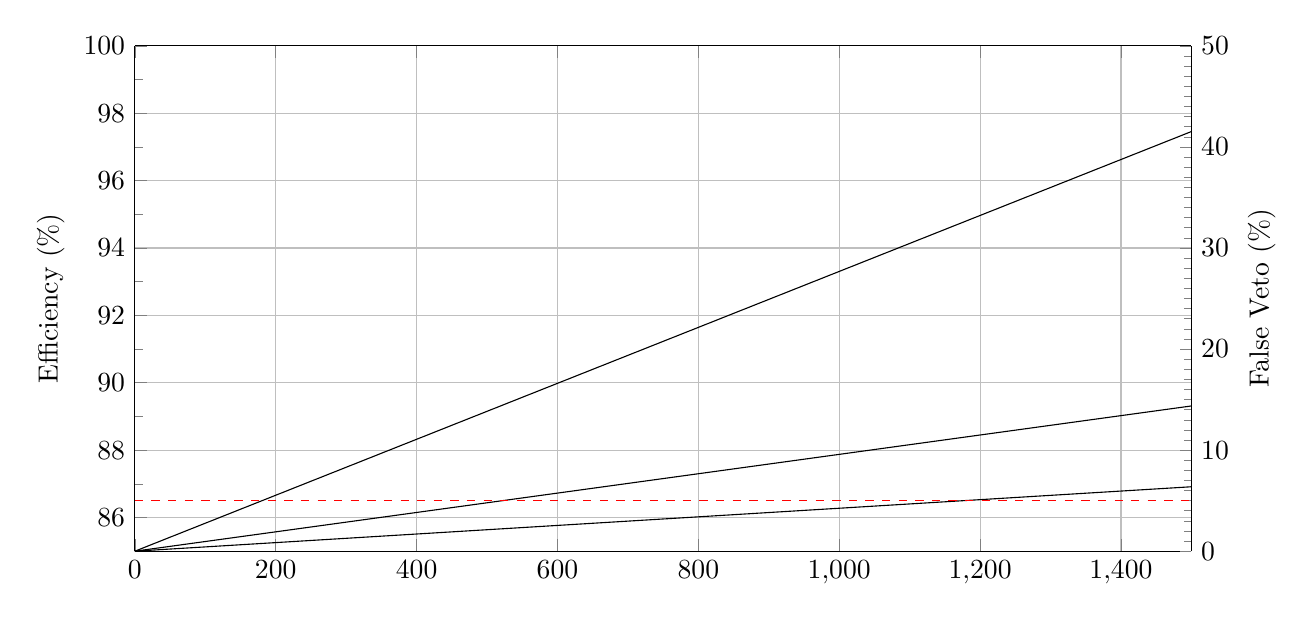
\begin{tikzpicture}
\centering
    \begin{axis}[
            ylabel=Efficiency (\%),
            width=15cm,
            height=8cm,
            grid=major,
            axis y line*=left,
            xmin=0, xmax=1500,
            ymin=85, ymax=100,
            minor y tick num=1,
            ]
    \end{axis}
    \begin{axis}[
            ylabel=False Veto (\%),
            yticklabel pos=right,
            axis y line*=right,
            axis x line=none,
            width=15cm,
            height=8cm,
            %grid=major,
            xmin=0, xmax=1500,
            ymin=0, ymax=50,
            minor y tick num=9,]
        \addplot[domain=0:1500,
            samples=3,
            ]
            {x * 42.5 * 100 / 1000000};
        \addplot[domain=0:1500,
            samples=3,
            ]
            {x * 95.8 * 100 / 1000000};        
        \addplot[domain=0:1500,
            samples=3,
            ]
            {x * 276.8 * 100 / 1000000};  
         \addplot[dashed, mark=none, red] coordinates {(0,5) (1500,5)};
    \end{axis}
            
\end{tikzpicture}
    \caption{Neutron tagging efficiency from AmLi at each height for the 200keV phe threshold}
    \label{fig:commissioning_amli_efficiency_with_bg_rate}
\end{figure}


\subsection{Neutron Captures}
\par
Another source that can be used to study the neutron capture time is the ${}^{252}{Cf}$ calibration source.
Spontaneous fission of ${}^{252}{Cf}$ typically results in a number of $\gamma$'s with a combined energy of up to 10MeV which are accompanied by a number of neutrons.
An example event from the LZ calibration run pre-SR1 is shown in Figure \ref{fig:cf252_event_viewer}.
This allows for neutrons to be tagged by tagging the fission by coincident $\gamma$'s in a each detector, and assuming later pulses are dominated by neutrons.

\begin{figure}[!htbp]
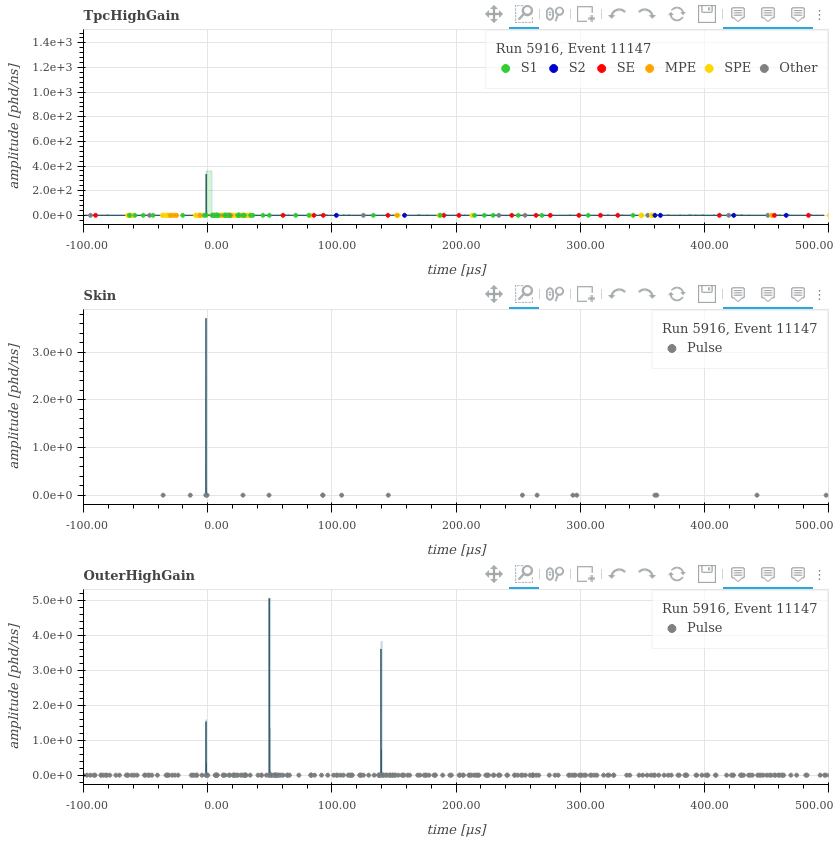
\includegraphics[width=10cm]{Figures/NeutronCaptureTime/cf252_eventviewer_5916.png}
\centering
\caption{Example event from ${}^{252}{Cf}$ calibration run showing the $\gamma$'s causing coincident pulses in each detector followed by two neutrons being captured in the Outer Detector}
\label{fig:cf252_event_viewer}
\end{figure}

\par
Although Figure \ref{fig:cf252_event_viewer} indicates that prompt $\gamma$'s can be used for tagging it does come with a significant caveat; namely that expressed in Figure \ref{fig:fission_fragments_time}.
There is a non-insignificant probability that $\gamma$'s will be emitted at the same time as a $\gamma$ from a neutron capture is released.
Additionally the majority of study into prompt $\gamma$'s from fission focus on the first 100ns post-fission and the energy and multiplicity beyond that time is not well theorised. 
However, by selecting events which only have a double or triple detector coincidence this can be mitigated.


\begin{figure}[!htbp]
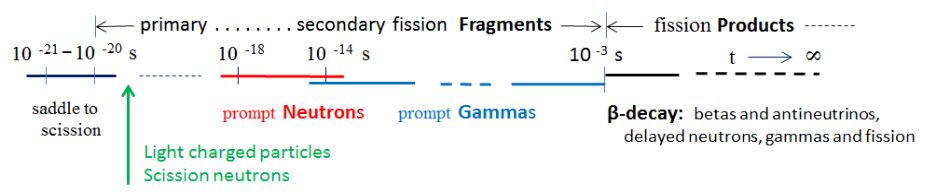
\includegraphics[width=13cm]{Figures/NeutronCaptureTime/fission_fragment_times.png}
\centering
\caption{Emission time-frame of fission components. Adapted from \cite{cf252_fission_ref}}
\label{fig:fission_fragments_time}
\end{figure}



\par
For the other neutron calibration sources, DD and AmLi, the same neutron tagging as described in Section XXX was used, where the NR band is isolated.
The result of this search is shown in figure XXX - overlaid is the neutron capture sim in the simulations.
What is apparent is that there is more than one exponential decays in data.
The simplest explanation is that a portion of the neutrons are being captured on H in either the water or acrylic that is between the source and GdLS.
In this case, the capture constant would be 220$\mu$s.
Initially this was excluded by selecting pulses above the H-peak, selecting events above 500phd.
However, as can be seen in Figure XXX, at least two exponents remain.
A fit was performed on each of the calibration sources separately, to equation XXX, and the results are summarised in Table \ref{tab:neutron_capture_times}.
\begin{table}[!htbp]
    \centering
    \begin{tabular}{c|c}
        Source            &  \\ \hline
        AmLi (CSD1 700mm) & \\ 
        DD                & \\
        ${}^{252}{Cf}$    &
    \end{tabular}
    \caption{Neutron capture time on Gadolinium isotopes in GdLS}
    \label{tab:neutron_capture_times}
\end{table}

Given that these neutrons are captured releasing in excess of 3MeV, they will have been captured by a Gd-isotope. 
Therefore what is being observed is most likely that the neutron bounces around in the acrylic, which would likely capture after 220$\mu$s before entering the GdLS to be captured.
This effect was observed in TODO CITE XXX so is reasonable that it would be seen here as well.
It could be validated deploying the calibration sources in a number of different locations where the thickness of the acrylic differs, this study may be possible pre-SR2.


\par
The GdLS cocktail used by LZ is similar to that of the DayaBay experiment, and as such, the neutron capture properties should be similar.
Using Equation XXX which is an extended version of that from DayaBay \cite{Dayabay_neutron_capture_fit_ref} was used to fit to both the thermalisation peak and the subsequent captures.

\begin{equation}
    N = Y
\end{equation}

